%% abtex2-modelo-artigo.tex, v-1.7.1 laurocesar
%% Copyright 2012-2013 by abnTeX2 group at http://abntex2.googlecode.com/ 
%%
%% This work may be distributed and/or modified under the
%% conditions of the LaTeX Project Public License, either version 1.3
%% of this license or (at your option) any later version.
%% The latest version of this license is in
%%   http://www.latex-project.org/lppl.txt
%% and version 1.3 or later is part of all distributions of LaTeX
%% version 2005/12/01 or later.
%%
%% This work has the LPPL maintenance status `maintained'.
%% 
%% The Current Maintainer of this work is the abnTeX2 team, led
%% by Lauro César Araujo. Further information are available on 
%% http://abntex2.googlecode.com/
%%
%% This work consists of the files abntex2-modelo-artigo.tex and
%% abntex2-modelo-references.bib
%%

% ------------------------------------------------------------------------
% ------------------------------------------------------------------------
% abnTeX2: Modelo de Artigo Acadêmico em conformidade com
% ABNT NBR 6022:2003: Informação e documentação - Artigo em publicação 
% periódica científica impressa - Apresentação
% ------------------------------------------------------------------------
% ------------------------------------------------------------------------

\documentclass[
	% -- opções da classe memoir --
	article,			% indica que é um artigo acadêmico
	11pt,				% tamanho da fonte
	oneside,			% para impressão apenas no verso. Oposto a twoside
	a4paper,			% tamanho do papel. 
	% -- opções da classe abntex2 --
	%chapter=TITLE,		% títulos de capítulos convertidos em letras maiúsculas
	%section=TITLE,		% títulos de seções convertidos em letras maiúsculas
	%subsection=TITLE,	% títulos de subseções convertidos em letras maiúsculas
	%subsubsection=TITLE % títulos de subsubseções convertidos em letras maiúsculas
	% -- opções do pacote babel --
	english,			% idioma adicional para hifenização
	brazil,				% o último idioma é o principal do documento
	]{abntex2}


% ---
% PACOTES
% ---

% ---
% Pacotes fundamentais 
% ---
\usepackage{cmap}				% Mapear caracteres especiais no PDF
\usepackage{lmodern}			% Usa a fonte Latin Modern
\usepackage[T1]{fontenc}		% Selecao de codigos de fonte.
\usepackage[utf8]{inputenc}		% Codificacao do documento (conversão automática dos acentos)
\usepackage{indentfirst}		% Indenta o primeiro parágrafo de cada seção.
\usepackage{nomencl} 			% Lista de simbolos
\usepackage{color}				% Controle das cores
\usepackage{graphicx}			% Inclusão de gráficos
% ---
		
% ---
% Pacotes adicionais, usados apenas no âmbito do Modelo Canônico do abnteX2
% ---
\usepackage{lipsum}				% para geração de dummy text
% ---
		
% ---
% Pacotes de citações
% ---
\usepackage[brazilian,hyperpageref]{backref}	 % Paginas com as citações na bibl
\usepackage[alf]{abntex2cite}	% Citações padrão ABNT
% ---

% ---
% Configurações do pacote backref
% Usado sem a opção hyperpageref de backref
\renewcommand{\backrefpagesname}{Citado na(s) página(s):~}
% Texto padrão antes do número das páginas
\renewcommand{\backref}{}
% Define os textos da citação
\renewcommand*{\backrefalt}[4]{
	\ifcase #1 %
		Nenhuma citação no texto.%
	\or
		Citado na página #2.%
	\else
		Citado #1 vezes nas páginas #2.%
	\fi}%
% ---

% ---
% Informações de dados para CAPA e FOLHA DE ROSTO
% ---
\titulo{Implementação de Governança de TI na Autarquia Federal Agência Espacial Brasileira }
\autor{Túlio Mendes Eiras\thanks{tulioeiras@gmail.com} \and César Augusto Borges de Andrade \thanks{caborges72@gmail.com}}
\local{Brasil}
\data{Faculdade FORTIUM - Especialização em Gestão de TI na Administração Pública\\
  SGAS Quadra 616 Módulo 114, Asa Sul - Brasília/DF - CEP 70.200-760 \\ 21 de Janeiro de 2015, v 1.2}
% ---

% ---
% Configurações de aparência do PDF final

% alterando o aspecto da cor azul
\definecolor{blue}{RGB}{41,5,195}

% informações do PDF
\makeatletter
\hypersetup{
     	%pagebackref=true,
		pdftitle={\@title}, 
		pdfauthor={\@author},
    	pdfsubject={Implantação de Governança de TI na Autarquia Federal Agência Espacial Brasileira},
	    pdfcreator={Tulio with César},
		pdfkeywords={abnt}{latex}{abntex}{abntex2}{atigo científico}, 
		colorlinks=false,       		% false: boxed links; true: colored links
  %  	linkcolor=blue,          	% color of internal links
   %	citecolor=blue,        		% color of links to bibliography
    %	filecolor=magenta,      		% color of file links
	%	urlcolor=blue,
	%	bookmarksdepth=4
}
\makeatother
% --- 

% ---
% compila o indice
% ---
\makeindex
% ---

% ---
% Altera as margens padrões
% ---
\setlrmarginsandblock{3cm}{3cm}{*}
\setulmarginsandblock{3cm}{3cm}{*}
\checkandfixthelayout
% ---

% --- 
% Espaçamentos entre linhas e parágrafos 
% --- 

% O tamanho do parágrafo é dado por:
\setlength{\parindent}{1.3cm}

% Controle do espaçamento entre um parágrafo e outro:
\setlength{\parskip}{0.2cm}  % tente também \onelineskip

% Espaçamento simples
\SingleSpacing

% ----
% Início do documento
% ----
\begin{document}

% Retira espaço extra obsoleto entre as frases.
\frenchspacing 

% ----------------------------------------------------------
% ELEMENTOS PRÉ-TEXTUAIS
% ----------------------------------------------------------

%---
%
% Se desejar escrever o artigo em duas colunas, descomente a linha abaixo
% e a linha com o texto ``FIM DE ARTIGO EM DUAS COLUNAS''.
% \twocolumn[    		% INICIO DE ARTIGO EM DUAS COLUNAS
%
%---
% página de titulo
\maketitle
\renewcommand{\resumoname}{Abstract}
\begin{resumoumacoluna}
 \begin{otherlanguage*}{english}
This article discusses an implementation suggestion of IT governance in the Brazilian Space Agency. With the main objective to sensitize senior management to invest in aligning IT to the business. By analyzing the institution identified the need to enhance the services provided by IT, in which an operation plan with tasks and goals is presented. The proposed plan contains some actions to be performed, including the organizational restructuring of IT. The proposed guidelines can be implemented by any institution that wants to transform your IT.

   \vspace{\onelineskip}
 
   \noindent
   \textbf{Key-words}: Governance Corporation, IT Governance, iGovIT, Deploy Governance, PMBoK, IT in Public Administration.
 \end{otherlanguage*}  
\end{resumoumacoluna}

% resumo em português
\renewcommand{\resumoname}{Resumo}
\begin{resumoumacoluna}
  Este artigo aborda uma sugestão de implementação de Governança de TI na Agência Espacial Brasileira. Com o objetivo principal de sensibilizar a Alta Administração a investir no alinhamento da TI ao negócio. Ao analisar a instituição identificou-se á necessidade de aprimorar os serviços prestados pela TI, no qual é apresentado um plano de operação contendo tarefas e metas. O plano proposto contém algumas ações a serem executadas, entre elas a reestrutura organizacional da TI. O roteiro proposto poderá ser implementado por qualquer instituição que queira transformar o quadro da TI.
  
\vspace{\onelineskip}

\noindent \textbf{Palavras-Chave}:Governança Corporativa, Governança de TI, iGovTI, Implantar Governança, PMBoK, TI na Administração pública.
\end{resumoumacoluna}

% ]  				% FIM DE ARTIGO EM DUAS COLUNAS
% ---

% ----------------------------------------------------------
% ELEMENTOS TEXTUAIS
% ----------------------------------------------------------
\textual

% ----------------------------------------------------------
% Introdução
% ----------------------------------------------------------
%\section*{Introdução}

\include{introducao}

\section{Conceitos Básicos} \label{first:figs}

 Segundo \cite{adm} toda organização existe para atende a um objetivo específico sendo pública ou privada. Existe um alvo de mercado a ser alcançado em que a junção de recursos físicos e humanos contribuem para sua execução. Ainda de acordo com \cite{adm} a composição de uma organização há responsabilidades que são inerentes a níveis hierárquicos. Podemos identifica-las nos seguintes grupos: 

\begin{enumerate}
\item Governação Corporativa - responsável pela tomada de decisão, elaborar metas, autorizar investimentos, fiscalizar atividades, dentre outros;
\item Gestão Administrativa - resposável por intermedia a Governança Corporativa com Operacional, gerenciar projetos e produtos, gerir indicadores, dentre outros; e
\item Operacional - responsável pela execução dos projetos e trabalhos operacionais.
\end{enumerate}

Os gurpos se interagem entre sí, de acordo com \cite{IBGC} e \cite{ImplantandoGTI:2012} a Governança Corporativa é responsável por traçar os objetivos, colher os resultados e auditar-lo. Para se alcançar resultados satifátorios é necessário a otimização dos processos e redução das redundâncias dos trabalhos, no qual se torna necessário a utilização da TI. A TI como disciplina precisa ser integrada a Governança Corporotativa como ferramenta meio no alcance dos resultados, que surge então a Governança de TI - GTI.
 
Para falarmos de Governança de TI, iremos abordar primeiramente a Governança Corporativa e sua principais características.

\subsection{Governança Corporativa}
Segundo \cite{IBGC} Governança Corporativa é:

\begin{quote}
	``Sistema pela qual as sociedades são dirigidas, monitoradas e incentivadas, envolvendo o relacionamento entre proprietários, Conselho de Administração, Diretoria e órgãos de controle interno. As boas práticas de governança corporativa convertem princípios em recomendações objetivas alinhando interesses com a finalidade de preservar e otimizar o valor da organização, facilitando seu acesso ao capital e contribuindo para a sua longevidade." \cite[p.17]{IBGC}
\end{quote}


De acordo com o \cite{IBGC} os princípios de Governança Corporativa são, transparência, equidade, prestação de contas e responsabilidade corporativa.

\textbf{Transparência} trata de diceminar a informação de resultados e ações. 

\textbf{Equidade} destaca tratamento igualitário a todos os acionistas. 

\textbf{Prestação de contas} trata da responsabilização de seus atos e omissões. 

\textbf{Responsabilidades corporativas} refere que os agentes de governança, devem zelar pela sustentabilidade das organizações contribuindo por sua longevidade.

A governança corporativa é composta pelo conselho de administração, conselho fiscal e auditoria independente. Todos fazem parte da tomada de decisão sobre os investimentos e projetos que alcançam seus objetivos. Nos órgãos federais a composição da governança corporativa são: o povo, os órgãos auditores e a administração de cada órgão.

	
\subsection{Governança de TI - GTI} \label{sec:govti}

A Governança de TI - GTI, baseado na \cite{GTI:TCU} e \cite{ImplantandoGTI:2012}, é o sistema pelo qual o uso atual e futuro da TI são dirigidos e controlados pela Governança Corporativa para garantir que a TI sustente, monitore, e estenda as estratégias e objetivos de negócio da organização. 

De acordo com \cite{ImplantandoGTI:2012}, são competências da Governança de TI: 

\begin{enumerate}
\item Prover o alinhamento estratégico da TI ao negócio;
\item Prover ferramentas que garantam a continuidade do negócio contra interrupções e falhas;
\item Prover junto a áreas de controle o alinhamento a regulamentos e normas internas e externas ao órgão.

\end{enumerate}

Os objetivos da GTI são inerentes ao negócio, o principal segundo \cite{ImplantandoGTI:2012}, é alinhar a TI aos requisitos do negócio, que inclui, soluções de apoio a tomada de decisões e apoio aos processos do negócio. O último proporciona garantia da continuidade dos serviços e a minimização da exposição do negócio aos riscos de TI. 

Ao aplicar a Governança de TI encontra-se dentro do principal objetivo, vários outros relacionados a GTI, que atendem as necessidades da organização. São eles:  

\begin{enumerate}
\item Traduzir as estratégias de negócio em plano para sistemas, aplicações, soluções, processos e infraestrutura, desenvolvimento de competências, estratégias de sourcing e de segurança da informação, dentre outras;
\item Prover o alinhamento e priorização da iniciativas de TI com a estratégia do negócio em um portifólio de TI que liga a estratégia e as ações do dia a dia;
\item Alinha a arquitetura de TI planejar os projetos e priorizá-los no presente e no futuro;
\item Prover a implantação de melhoria nos processos operacional e de gestão necessários para atender aos serviços de TI.
\end{enumerate}

Essas atividades levam a TI tomar um rumo alinhado as necessidade da organização, sem desperdiçar o potencial que a TI proporciona e assim adicionando valor ao negócio.

Segundo \cite{GTI:TCU}, a Governança de TI tem foco no direcionamento e monitoramento das práticas de gestão e uso da TI de uma organização, tendo como indutor e principal beneficiário a alta administração da instituição.

O objetivo de negócio da organização deve ser identificado e repassado a TI, para que possa criar estratégias e técnicas, utilizando  metodologias disponíveis no mercado para alcançá-los. 

A governança de TI como disciplina não segue solitária na busca da valorização da TI. Existem vários modelos de referência que abordam a TI em sua totalidade, como:

 \begin{itemize}
 
 \item ISO/IEC 38500 - Trata de fornecer uma estrutura de princípios para os dirigentes utilizarem na avaliação, no gerenciamento e no monitoramento do uso da TI em suas organizações. 
 \item CobiT - Trata em contribuir para o sucesso da entrega de produtos e serviços de TI a partir da perspectiva das necessidades do negócio, com um foco mais acentuado no controle que na execução.
 \item Val IT - Trata de um modelo que reforça a necessidade de demonstração do retorno que a TI fornece ao negócio.
 \item Risck IT - O modelo é dedicado a auxiliar no gerenciamento de riscos relacionados a TI.
  
 \end{itemize}
 

\subsection{Governança de TI na Administração Pública}

Segundo \cite{ImplantandoGTI:2012} e \cite{SISP} , A partir da década de 90 o governo federal identificou a necessidade de organizar e investir na implementação de GTI em seus órgãos. Foi então que criou o Sistema de Administração de Recursos de Informação e Informática (SISP), com o objetivo de organizar a operação, o controle, a supervisão e coordenação dos recursos de informática da Administração direta, autárquica e fundacional do poder executivo Federal. 

O SISP é responsável por direcionar os órgão federais a alcançar alinhamento estratégico. Já aspectos referentes a segurança da informação no Governo Federal é de responsabilidade do Gabinete de Segurança Institucional da  Presidência da República, através do Departamento de Segurança da Informação e Comunicações. A fiscalização da tecnologia da informação da Administração Pública Federal e de responsabilidade do Tribunal de Contas da União - TCU.

Essas instituições auxiliam os órgãos federais a promoverem o poder alcançado pela valorização da TI na Administração, pois a administração necessita fornecer serviços com qualidade e segurança a sociedade. 

\subsection{Índice de Governança de TI - iGovTI}\label{subsec:iGovTI}

Segundo \cite{acordaoTCU}, o TCU com o objetivo de avaliar a situação da Governança de TI na Administração Pública Federal, tem realizado levantamento baseado em questionários que abordam práticas de governança e de gestão de TI previstas em leis, regulamentos, normas técnicas e modelos internacionais de boas práticas. 

Esse levantamento é feito desde 2007 e tem o objetivo de acompanhar e manter as informações atualizadas com a situação da governança de tecnologia da informação na Administração Pública Federal - APF.
 
De acordo com \cite{acordaoTCU} o Índice de Governança de TI - iGovTI foi criado em 2010 pelo TCU com o propósito de orientar as organizações públicas no esforço de melhoria da governança e da gestão de TI. O índice tambem permite a avaliação, de um modo geral, a efetividade das ações adotadas para induzir a melhoria da situação de governança de TI na APF.   

Por meio de questionário e a consolidação das respostas recebemos como resultado o iGovTI. As organizações que respondem ao questionário são classificadas e seguimentadas de acordo com perfil, para facilitar a identificação da situação no índice.

\section{Trabalhos Relacionados} \label{ses:rela}

A Governança de TI no âmbito federal, é caracterizada por ser uma busca constante pelos órgãos, haja visto que a TI esta em constante inovação.

Foi realizado uma pesquisa em alguns órgãos do Governo Federal da visão de cada um sobre a TI. 

\subsection{Tribunal de Contas da União}

Segundo o \cite{GTI:TCU}, o TCU entende que por ser uma instituição que depende de informação para a realização de seus trabalhos e cada vez mais da TI para adequadamente tratar, analisar, fazer uso, disseminar e proteger essas informações. Além disso, é cada vez maior a automação de processos de trabalho do Tribunal, como meio de se assegurar o alcance e a manutenção de padrões de desempenho e qualidade compatíveis com as necessidades da sociedade brasileira.

Como visto o órgão valoriza a informação, pois os frutos de seus trabalhos dependem do tratamento dessas informações. Quem faz o tratamento e a manipulação é a própria TI, atravéz dos diversos sistemas que foram criados a partir de otimização dos processos.

A Governança de TI do TCU está justamente atrelado a esse objetivo de gerir a informação, que é alem da otimização dos processos, é sim usar os benefício que a informação apresenta pela tecnologia da informação para adicionar valor ao negócio.  

\subsection{Caixa Economica Federal - CEF}

Por se tratar de uma instituição financeira nacional, a CEF precisa suportar as atividades seguras e competitiva para se manter no mercado. Pelo fato de trabalhar com alto capital e varios concorrentes do mercado financeiro.

Com esses atributos a instituição tem segundo \cite{Caixa}, objetivos de Governança de TI bem definidos de eficiência na entrega de soluções de TI, ser inovador nas soluções em TI e ter disponibilidade e performance nos serviços de TI. Esses que contribuem com os objetivos de negócio de liderar acesso a serviços financeiros, maximizar eficiência operacional e de ser o principal agente financeiro do desenvolvimento sustentável brasileiro.

A CEF é uma instituição madura na Governança de TI pois identifica os benefícios da TI desde 1996, época em que começou a investir em TI alinhando as sua estratégias em projetos de TI.  
 
 \subsection{Banco Central do Brasil - Bacen}
 
 Banco central responsável por fiscalizar as instituições financeiras do país é uma referência para os demais órgãos federais na gestão da Governança de TI. 
 
 Segundo \cite{Bacen} antes da implantação de GTI o órgão passava por situações indesejadas na execução das atividades de TI. Tais com projetos com elevados prazos e entrega, atrasos na entrega de projetos, baixa percepção da qualidade dos serviços de TI e baixa precisão dos esforços realizados. Um cenário crítico para uma instituição com grandes responsabilidades. 
 
 Então focaram em otimizar esses processo na adoção de boas práticas para gerência de projetos e serviços. 
 
 Para a gerência de projetos foi adotado como referência o PMBok, com o objetivo de otimização processos de replanejamento, acompanhamento e definição de indicadores de desempenho.
 
 Para a gerência de serviços foi adotado como referência o, Information Technology Infrastructure Library -ITIL. Que ajudou nos processos de gestão de mudanças e incidentes e na definição de indicadores de disponibilidade.
 
 Esses atributos são evidências da implantação de Governança de TI no Bacen, pois os serviços e projetos que o órgão trabalha são voltados a facilitação e otimização das diretrizes e tarefas estabelecidas a ele. Além do alinhamento da TI ao negócio, as ferramentas auxiliam a tomada de decisão através do portifólio de projetos.
 
 
	
\section{Cenário Atual}\label{aeb}

A Agência Espacial Brasileira - AEB, autarquia federal vinculada ao Ministério da Ciência e Tecnologia e Inovação - MCTI, criada em 1994, tem a finalidade de promover o desenvolvimento das atividades espaciais de interesse nacional. Compete a ela também dentre vários outras atividades, a formulação e coordenação da política espacial brasileira, de acordo com \cite{Lei:8.854} e \cite{Decreto:4.718}.

Segundo \cite{Decreto:4.718}, a AEB é um dos órgãos que compõem o Sistema Nacional de Desenvolvimento das Atividades Espaciais - SINDAE, que é o conjunto dos órgãos responsáveis pela organização e execução das atividades do Programa Espacial Brasileiro.

As iniciativas e atividades planejadas e em execução pela autarquia, estão organizadas pelo Programa Nacional de Atividades Espaciais - PNAE.

A estrutura organizacional da AEB disponível na Figura~\ref{fig:OrgAeb}.

\begin{figure}[ht]
\centering
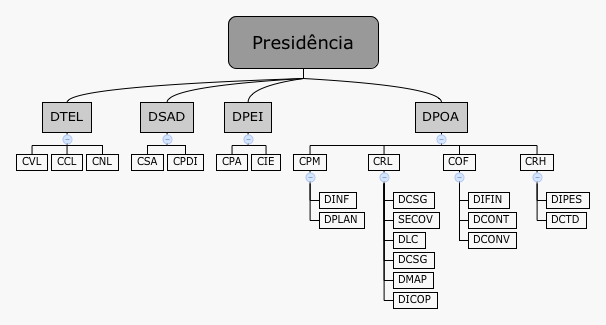
\includegraphics[width=.7\textwidth]{OrgAeb.png}
\caption{Organograma AEB}
\label{fig:OrgAeb}
\end{figure}

A agencia está subdividida em: presidência, diretorias, coordenações e divisões. As diretorias são responsáveis por executar as tarefas do órgão, e segmenta suas atividades na coordenações e divisões. Compete as diretorias de acordo com o \cite{Decreto:4.718}:

\textbf{DTEL} - Diretoria de Transporte Espacial e Licenciamento, compete a diretoria implementar, coordenar e supervisionar projetos e atividades relativos a foguetes, veículos lançadores e centros de lançamento. Como também promover iniciativas de comercialização de bens e serviços espaciais, coordenar a concessão de licenças e autorizações relativas as atividades espaciais. 

\textbf{DSAD} - Diretoria de Satélites, Aplicações e Desenvolvimento, a diretoria é responsável por implementar coordenar e supervisionar os projetos e atividades relativos a satélites espaciais, como também promover a transferência de tecnologia para setor produtivo e promover a integração de instituições de ensino e sua capacitação para atuar em atividades espaciais.
 
\textbf{DPEI} - Diretoria de Política Espacial e Investimentos Estratégicos, compete a diretoria elaboração e atualização do PNAE, identificação de oportunidades e estratégias de investimento no setor espacial e realizar estudos e análises pertinentes à área espacial.

\textbf{DPOA} - Diretoria de Planejamento Orçamento e Administração, a diretoria é responsável por coordenar e controlar a execução das atividade relacionadas aos Sistemas de Pessoal Civil da Administração Federal - SIPEC, de Organização e Modernização Administrativa - SOMAD, de Administração dos Recursos de Informação e Informática - SISP, de Serviços Gerais - SISG, de Planejamento e de Orçamento Federal, de Contabilidade Federal e de Administração Financeira Federal.

Como podemos observar a diretoria responsável pela área de TI é a, DPOA diretoria responsável pela área administrativa do órgão.

\subsection{Tecnologia da Informação - TI da AEB}\label{sec:TIAEB}

A Divisão de Informática - DINF, é subordinada a Coordenação de Planejamento e Modernização - CPM que pertence a DPOA. A divisão é a área responsável por fornecer serviços de TI, e pela gerência dos projetos e atividades relacionadas a TI, desde suporte ao usuário a aquisição de materiais de informática.

A DINF está organizada como mostra a Figura~\ref{fig:orgDinf}.

\begin{figure}[ht]
\centering
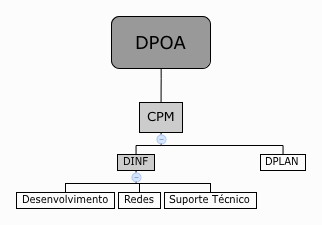
\includegraphics[width=.7\textwidth]{DPOA_dinfAtual.png}
\caption{Organograma DINF}
\label{fig:orgDinf}
\end{figure}

Compete a DINF:

\begin{itemize}
\item Manter Plano Diretor de TI - PDTI;
\item Implementação de metodologias e ferramentas indicadas pelo SISP;
\item Gerência de Informação;
\item Suporte a usuário;
\item Desenvolvimento e manutenção de sistemas administrativos;
\item Desenvolvimento e manutenção de Sitio e Intrnaet da AEB;
\item Análise de viabilidade de implementação de tecnologia;
\item Gerência de redes;
\item Desenvolvimento e manutenção de projetos de redes;
\item Responsável pela implementação de política de segurança digital e 
\item Aquisição de recursos de informática.
\end{itemize}

\subsubsection{iGovTI}

Segundo a definição de IGovTI na Sesão \ref{subsec:iGovTI} o índice avalia a efetividade das ações para medir a Governança de TI nos orãos federais. 

A AEB participa dessa avaliação no qual os resultado vem avançando no indice.  Segundo o \cite{acordaoTCU} os últimos resultados foram:

iGovTI 2012 com 349 participantes foi:

\begin{itemize}
\item 8º lugar, dentre 23 autarquias do governo federal
\item 73º lugar, dentre 214 órgãos do governo federal vinculados ao SISP/MPOG
\item 149º lugar, dentre 349 órgãos do governo federal
\end{itemize}

iGovTI 2014 com 372 participantes é:

\begin{itemize}
\item 7º lugar, dentre 27 autarquias do governo federal
\item 54º lugar, dentre 229 órgãos do governo federal vinculados ao SISP/MPOG
\item 105º lugar, dentre 372 órgãos do governo federal
\end{itemize}

Este índice ajuda a instituição mensurar a importância que a TI exerce no órgão quanto a sua governança e gestão.

\subsection{Cenário Encontrados}

Como já dito na Seção \ref{first:figs}, a TI precisa ser alinhada as estratégias das instituições para que haja alcance satisfatório nos resultados.

A informática na AEB é considerada área meio e é responsável por disponibilizar os serviços da TI aos usuários e os manter em funcionamento. Essa situação evidencia-se ao observar o organograma da DINF na Figura~\ref{fig:orgDinf}, onde as áreas que a compõem são: suporte a aplicação, a equipamentos e serviços que já são fornecidos. Não existe área responsável por identificar as necessidades do negócio, nem quanto a segurança dos dados. Nem existe área ou processo responsável em aplicar a gerência de resposta a riscos.

Alguns problemas existentes:

\begin{itemize}
\item Processos Indefinidos;
\item Recursos humanos insuficientes para atender as demandas;
\item Aplicações inconsistentes com as necessidades do órgão;
\item Falta de estabilidade de serviços fornecidos pela rede.
\end{itemize}

Esses serviços deixam a desejar não pela falta de mão de obra competente, mas pela falta de área responsável dedicada a cada uma das diversas atividades que a TI exerce. 

A dependência do negócio a TI é caracterizado por quanto maior a quantidade de operações chaves dependem da TI, maior é seu papel na organização. Como mostra a Figura~\ref{fig:impactoti} :

\begin{figure}[ht]
\centering
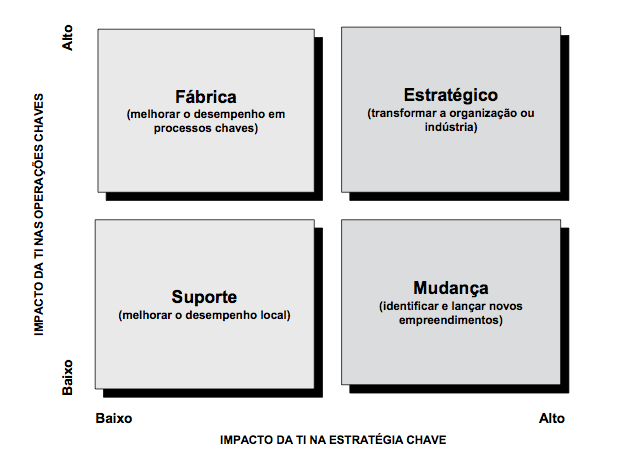
\includegraphics[width=.7\textwidth]{impactoTI.png}
\caption{Impacto estratégico da tecnologia da informação.}
\label{fig:impactoti}
\end{figure}

\begin{itemize}
\item Quando a TI tem alto impacto nas operações chaves e alto impacto nas estratégias chave, ela é estratégica ao negócio.
\item Quando a TI tem alto impacto nas operações chaves e baixo impacto nas estratégias chave, a TI depende do negócio mas o seu futuro não.
\item Quando a TI tem baixo impacto nas operações e alto impacto nas estratégias chave, está apoiando o direcionamento do futuro da organização.
\item Quando a TI tem baixo impacto nas operações chave e baixo impacto nas estratégias chave, a TI está executando tarefas de suporte.
\end{itemize}

Segundo a Figura~\ref{fig:impactoti} disponível em \cite{ImplantandoGTI:2012}, a TI encontrada na AEB é uma TI de suporte, pois tem um baixo valor em operações chave e baixo valor nas estratégias do negócio. É focada em atender demandas dos usuários e em manter os sistemas e seus serviços em funcionamento.


\section{Proposta de Implementação de Governança de TI}\label{sec:proposta}

Sabendo que a AEB é um órgão federal que presta serviços a sociedade brasileira, é ideal que o preste com  qualidade e eficiência. Mediante ao cenário exposto na Seção \ref{aeb}, identifica-se que a AEB necessita valorizar a TI para que possa usufruir de grandes benefícios a partir da TI.

Com a implementação da Governança de TI pode-se alcançar resultados concretos e benéficos ao órgão alinhando a TI ao negócio. Mas essa tarefa é complexa e demanda tempo para chegar a resultados satisfatórios, pode-se dizer que é um empreendimento de longo prazo.

 Segundo \cite{ImplantandoGTI:2012}, existem alguns requisitos que devem ser atendidos para sua implantação, como:

\textbf{Liderança para mudança}: instituir um executivo patrocinador que faz parte da alta direção do órgão, para assumir a liderança e garantir os fundos necessários para a implementação.

\textbf{Envolvimento dos executivos da organização}: Envolver os demais executivos do órgão, no caso as diretorias, pois são gestores de processos indispensáveis ao órgão e que podem ser atendidos pela TI.

\textbf{Atacar as principais vunerabilidades}: Deve haver identificação e priorização das principais vulnerabilidades pela Governança de TI, para obter resultados a curto prazo e sucesso do empreendimento. Os resultados obtidos devem ser comparados com anteriores para que as melhorias sejam evidenciadas.

\textbf{Ter uma abordagem de gestão de mudança cultural}: Ao implementar a GTI vão haver várias resistências envolvendo os funcionários da TI, os usuários e os clientes, pois haverão mudanças na execução dos trabalhos. Para isso deverá ser planejada a mudança cultural pela gerência e a presidência, que deverão tomar atitudes condizentes para a implementação.

\textbf{Equipe Qualificada}: Para implementar a GTI deve-se ter pessoas qualificadas e experientes que trabalham com planejamento, implementação e gerencie o processo de implementação.

\textbf{Certificar se os benefícios da implementação de GTI estão sendo atingidos}: A Alta administração só entenderá os esforços que estão sendo investidos se houver retornos visíveis, numéricos e em especial agregar valor ao negócio.


\subsection{Roteiro de Implementação de Governança de TI}

Para implementar está proposta de governança de TI segundo \cite{ImplantandoGTI:2012} é necessário seguir algumas atividades que são de grande importância para obter resultado. A Figura~\ref{fig:roteiro} mostra um roteiro a ser seguido para a implementação da GTI.

\begin{figure}[ht]
\centering
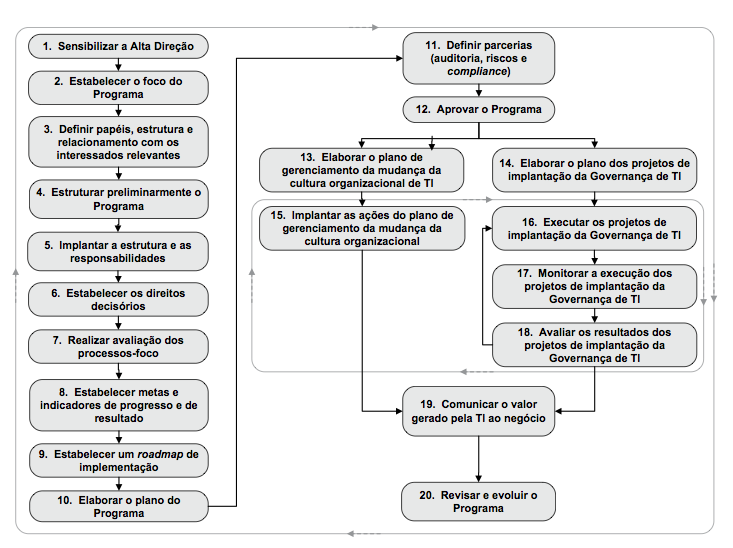
\includegraphics[width=1.0\textwidth]{roteiro.png}
\caption{Proposta de roteiro para implementação de Governança de TI.}
\label{fig:roteiro}
\end{figure}

O roteiro norteia as atividades que deve-se seguir para obter a governança de TI no órgão. Seguiu-se algumas aplicando em dados encontrados no ambiente da AEB. Esse roteiro é complexo e demanda vários ciclos de tarefas para seu êxito. Sugeri-se em algumas delas, atividades que podem ser executadas durante a implementação da GTI, mas em outras foi realizada contextualização da sua importância no processo de implementação da GTI.

\subsubsection{Sensibilizar a Alta Administração}

Sensibilizar a alta direção quanto a importância da TI para o órgão, pois sem seu apoio e patrocínio serão impossíveis. 

A TI na AEB está passando por alguns problemas que podem ser resolvidos com investimentos adequados. Um dos mais importância são os relacionados a segurança dos dados, pois o órgão lida com informações de sigilo como tratados, acordos, dados financeiros, emails organizacional e dados pessoais. Essas informações precisam ser protegidas, em especial nos dias de hoje onde foram evidenciadas espionagens por países vizinhos, apartir de vulnerabilidade ligadas a TI.

Para que a TI esteja alinhada as estratégias do órgão é necessaria a priorização de investimentos em projetos que partiram da tomada de decisão da alta administração.

Os processos de atividades administrativas precisam ser mapeadas e otimizados para que haja uma maior transparência de informações a alto administração.

Com a utilização de metodologias de boas práticas que a TI se baseia, referidas na Seção \ref{sec:govti}, pode-se obter resultados satisfatórios de utilização da TI.

\subsubsection{Objetivos de Implementação da GTI }

Com a aplicação da governança de TI queremos inicialmente identificar os processos e gaps organizacionais para que possa encontrar estratégias em sua otimização.

O Segundo é aplicação de ferramentas que  possibilita o gerenciamento e a transparência do andamento de projetos espaciais.

O terceiro é investir em ferramentas que auxiliam a tomada de decisão dos investimentos espaciais. A partir de informações e critérios atuais e históricos que serão cruzadas para disponibilização em dashboards.

O quarto é mater a continuação do serviço e preocupar-se com a segurança da informação.

\subsubsection{Estrutura da Diretoria de GTI}\label{subsec:estruturaGTI}

A AEB precisa de uma reestruturação na área de TI, foi visto na Seção \ref{sec:TIAEB} que a TI está em um posição abaixo do que costuma acontecer em órgãos federais, no qual a TI é tratada como uma diretoria responsável em agregar valor ao negócio.

Para então se implementar Governança de TI no órgão, deve ser criada uma diretoria responsável pela governança, coordenações e divisões responsáveis pela gerência e execução dos processos.

A Diretoria de Governança de TI será responsável por tomar decisão junto a presidência e as demais diretorias dos investimentos, projetos, contratações e aquisições que poderão ser atendidos pela TI. Analisar os resultados alcançados e identificar oportunidades. Implantar sistemas que atenda os processos do órgão assim como manter o funcionamento, implementar segurança de TI e atender as recomendações do SISP. Assim como fornecer suporte a infraestrutura e o atendimento ao usuário.

A Diretoria será dividida em quatro coordenações:

\textbf{Coordenação de Desenvolvimento} - Será responsável por implementar e manter as aplicações de projetos definidos pela GTI e manter os mecanismos de comunicação internos e externos do órgão, como Site e Intranet.

\textbf{Coordenação de Infraestrutura} - Será responsável por fornecer acesso as aplicações internas e externas através de redes computacionais, a manutenção de equipamentos e suporte ao usuário e a implementação da segurança de informação.

\textbf{Coordenação de Governança de TI} -A coordenação será responsável por mapear os processos, auxiliar na identificação das necessidades do órgão, gerenciar as aplicações, aplicar os modelos de boas práticas de mercado como: CobiT, Itil e PMBOK assim como as recomendações do SISP. E também implementar sistemas e ferramentas que auxiliam a tomada de decisão da alta administração por meio de Business iIntelligence - BI.

\textbf{Coordenação de Gerência de Recursos} - Será responsável por implementar e gerenciar contratos de recursos humanos das empresas que prestam serviço a diretoria, e recursos tecnológicos, assim como sua distribuição e fiscalização.

A Figura~\ref{fig:propostaOrg} contém a estrutura da diretoria proposta:

\begin{figure}[ht]
\centering
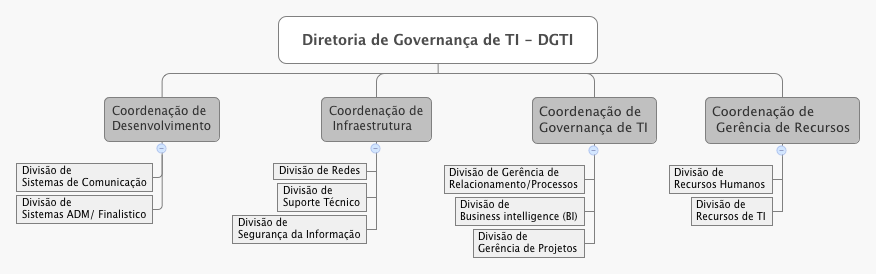
\includegraphics[width=1.0\textwidth]{DGTI.png}
\caption{Proposta de Estrutura Organizacional para GTI}
\label{fig:propostaOrg}
\end{figure}

\subsubsection{Programa de Governança de TI}

Segundo  \cite{ImplantandoGTI:2012}i e o \cite{PMBOK/PMI:2013}, programa é um grupo de projetos gerenciados de forma coordenada a obter benefícios que não estariam disponíveis se os projetos fossem gerenciados individualmente.

Os projetos envolvidos a TI serão gerenciados pela Coordenação de Governança de TI, serão classificados e gerenciados conjuntamente por programas específicos de acordo com o perfil dos projetos. De início sugerimos a criação de dois programas: o responsável por projetos da área meio que auxiliarão a processos administrativos; e os que possuirão projetos voltados a área espaciais que fazem parte da área fim.

\subsubsection{Direitos Decisórios}

O poder de decisão dos investimentos e prioridades serão da Diretoria de Governança de Ti, com participação dos diretores das demais áreas do órgão.  A diretoria de TI estabelecerá como os serviços são cobrados e os resultados desejáveis.

\subsubsection{Avaliação dos Processos}

Para melhorar a avaliação dos serviços prestados e identificar prioridades, foi feito um levantamento das opiniões dos usuários do órgão e chegamos as seguintes prioridades:

\begin{itemize}
\item Projeto de gerência dos recursos humanos, e recursos logísticos, integrado a sistemas fornecido pelo governo.
\item Projeto de gerência de documentos que possibilite uma maior manipulação.
\item Projeto de gerência de equipamento de TI integrado ao de recursos humanos.
\item Melhoria do atendimento ao usuário.
\item Fornecimento de serviços da rede na ausência de energia.
\item Melhoria na segurança das informações.
\end{itemize}

\subsubsection{Estabelecer Metas} \label{subsec:projetos}

Nesta seção, com base no processos identificados, serão definidas as metas.

Projetos ligados a área administrativa como gerência de recursos humanos, almoxarifado e equipamentos de TI, podem ser solucionados com aquisição de Enterprise Resource Planning - ERPs. Para esses projetos a primeira tarefa é estudar a viabilidade de implementação dos ERP. Caso não seja viável será realizada uma estratégia para desenvolvimento da solução no órgão.

O projeto de gerência de documentos já está implementado na casa, mas há a necessidade de incentivar a utilização do sistema na casa. A principal meta é incentivar os gestores a utilizarem e divulgar a solução a seus subordinados. A segunda é identificar as falhas do sistema e tratá-las.
 
A melhoria de atendimento ao usuário é uma atividade constante que não pode ser tratada como um projeto. A meta para essa atividade é implementar um sistema que possibilita a avaliação da TI em suas diversas tarefas, para que a gestão possa elaborar estratégias para melhorar os índices de serviços. 

Para o projeto de fornecimento de serviço da rede na ausência de energia, deverão adotar algumas estratégias. A primeira é aquisição de No Break e geradores para os servidores do prédio sede da rede. Assim com treinar os funcionários para gerênciá-los. 

O projeto de segurança da informação é um dos mais complexos pois além de vários processos envolvidos abrange a cultura organizacional. A primeira meta é mapear e elaborar planos de resposta as vulnerabilidade da TI do órgão. Como segunda seria a implementantação da política de segurança da informação.

\subsubsection{Estabelecer RoadMap de Implantação}

Essa seção trata a sequência, as interdependências, as melhorias e os benefícios a serem alcançados em cada projeto.

No projeto de automação de processos administrativos:

\textbf{Sequência:} Começara pelo levantamento de requisitos, mapeamento dos processos das atividades envolvidas. Logo após pesquisara de uma solução adequada para atender as necessidades e apresentaremos as propostas aos usuários e gestores. Por fim a elaboração do termo de referência para a aquisição da ferramenta e parametrização dos serviços.

\textbf{Interdependências:} O início do projeto depende necessariamente da autorização da governança. Após autorização se inicia o levantamento das necessidades e mapeamento dos processos. Logo após, a aquisição da ferramenta.

\textbf{Melhoria e benefícios:} O projeto otimizará os processos das áreas envolvidas, assim como transparência das informações disponíveis em formulários.

Projeto para gerência de documentos.

\textbf{Sequência:} A gerência de documentos já está implementada, o trabalho é de divulgação da ferramenta. As atividades são de identificar as áreas que utilizarão o sistema e divulgá-lo entre as diretorias. 

\textbf{Interdependências:} Primeiro será feito levantamento das áreas que consumirão o sistema e após isso a divulgação pelas diretorias.

\textbf{Melhoria e benefícios:} Com a divulgação o sistema passará a ser utilizado pelos usuários possibilitando uma maior gerência, pesquisas e substituirão espaços físicos utilizados para a lotação de arquivos.

Melhoria de atendimento ao usuário.

\textbf{Sequência:} A melhoria no atendimento ao usuário conterá as atividades de implementação de sistema de avaliação dos serviços de TI, monitoramento dos serviços resultantes e implementação de boas práticas para o atendimento.

\textbf{Interdependências:} Em primeiro lugar será implementado o sistema de avaliação, logo após serão analisados relatórios das avaliações e em seguida a implementação de boas práticas para sua melhoria. 

\textbf{Melhoria e benefícios:} A atividade contará de três passos que resultarão na otimização dos serviços e na identificação de gargalos.

Projeto de fornecimento de energia:

\textbf{Sequência:} As tarefas da continuidade dos serviços de rede após queda de energia são, aquisição de No Break, sua instalação, aquisição e instalação do gerador de energia para o bloco de lotação da rede e a capacitação dos funcionários para sua gerência. 

\textbf{Interdependências:} O primeiro será a aquisição do No Break. Segundo, a instalação e a aplicação de testes. O terceiro a aquisição do gerador do bloco da rede. Quarto é a capacitação dos funcionários na utilização dos equipamentos.

\textbf{Melhoria e benefícios:} Essas atividades possibilitarão a continuidade dos serviços de rede como sistemas internos, o site e a intranet em quedas de energia.

Implantação da Segurança da Informação:

\textbf{Sequência:} A implementação da Segurança de TI é um projeto complexo pois inicialmente precisa da sensibilização da governança corporativa. As atividades iniciais serão: a concientização da importância do investimento e implementação, levantar e planejar as ações da área e criar a política de segurança da informação.

\textbf{Interdependências:} A primeira atividade é a concientização da governança corporativa, o segundo é o planejamento de ações. O terceiro é a criação da política de segurança de TI.

\textbf{Melhoria e benefícios:} A criação da área  tornarão os serviços de TI mais completos identificando vulnerabilidades, evitando ataques externos, planejando respostas a riscos dentre outros benefícios.

\subsubsection{Plano do Programa de Governança de TI}

O Plano do Programa de Governança de TI conterá um esboço total descrevendo todos os atributos que determinam o sucesso do Programa de Governança.

Segundo \cite{ImplantandoGTI:2012}, são eles:

\begin{itemize}
\item Escopo do programa contendo os processos, estruturas e ações de TI a serem implementados.
\item Sequência de implementação dos processos, respeitando as considerações técnicas requeridas.
\item Linha de tempo prevista para implementação dos processos.
\item O plano de recursos estimados para o programa.
\item Os serviços a serem adquiridos.
\item O orçamento para o programa e para cada um dos projetos. 
\item Os benefícios esperados a serem atingidos, à medida que os processos forem sendo implementados.
\item Plano de gerênciamento do programa.
\item Estrutura de gestão do programa e a matriz de responsabilidades.
\item Riscos do programa.
\item Estratégia de gerência de mudanças.
\item Plano de continuidade do programa.
\item Critérios de qualidades a serem seguidos pelos projetos.
\item Métricas de progresso a serem consideradas pelos projetos componentes do programa.
\item Pontos de controle do programa.
\end{itemize}

Sugere-se que a AEB atente a todos os atributos para que possa ter bons resultados na implementação da Governança de TI e evitando surpresas desagradáveis.

\subsubsection{As Parcerias com Auditoria Interna e Externa}

Segundo o \cite{ImplantandoGTI:2012}, as áreas de auditoria interna e externa são grandes aliadas na implementação de Governança de TI pois têm acesso à Alto Administração. Parceria que se torna importante ao avaliar os processos e identificar as grandes vunerabilidades da TI para o negócio.

Essas informações são muito importantes para o período inicial da governança de TI, mas também durante seu curso. As áreas de auditorias são:

\begin{itemize}	
\item Auditoria Interna.
\item Tribunal de Contas da União - TCU.
\item Controladoria Geral da União - CGU.
\end{itemize}

A área responsável do órgão é a Auditoria Interna que fiscaliza se os processos estão de acordo com requisitos da governança e leis.

O TCU e a CGU se responsabilizam por fiscalizar o órgão como um todo, especialmente na utilização de boas práticas de execução dos projetos, fiscalização de contratos e conformidade com leis que regulamentam os setores.

\subsubsection{Aprovação do Programa}

A aprovação do programa de implementação de GTI, dependerá de autorização da Alto Administração. Na qual ao autorizar a execução do programa, automaticamente autorizará os projetos e recursos financeiros para sua implementação.

\subsubsection{Elaboração do Plano de Mudança da Cultura Organizacional}\label{sec:cultural} 

É necessário entender-se que para o sucesso da implntação da Governança de TI existem pontos chave que precisam ser trabalhados. que são os recursos humanos.

Para haver uma mudança na organização como a criação de uma nova diretoria será necessário elaborar um plano de mudança da cultura organizacional para se alcançar os objetivos desejados. 

Essa atividade demanda uma análise profunda dos processos organizacionais: pessoas, grupos de trabalhos e da estrutura organizacional.

 Portanto não falaremos do plano de mudança, mas sim da sua importância para o sucesso da Implantação da GTI.

A cultura organizacional de acordo com \cite{schein:1985} é:

"Cultura é a experiência que o grupo adquiriu à medida que resolveu seus problemas de adaptação externa e integração interna, e que funciona suficientemente bem para ser considerada válida. Portanto, essa experiência pode ser ensinada aos novos integrantes como forma correta de perceber, pensar e sentir-se em relação a esses problemas".

Ainda de acordo com o autor, para realmente interpretar a cultura de uma organização, deve se ir além dos artefatos visíveis e descobrir os pressupostos básicos fundamentais, que é, como são as relações do centro da cultura da organização. 

Para se aplicar a mudança cultural deve-se:
\begin{enumerate}
\item Avaliar a cultura organizacional atual e definir cultura desejada;
\item Avaliar as gaps entre a cultura atual e deseja;
\item Identificar ações e iniciativas para eliminar os gaps; 
\item Criação de um grupo de gerência de mudança com os líderes de TI da organização;
\item Plano de comunicação, para disseminar o projeto pelo órgão;
\item Programa de capacitação
\item Programa de desenvolvimento de liderança;
\item Estabelecimento de metas;
\item Recursos humanos e orçamentário;
\item Plano de ação com cronograma e responsabilidades.
\end{enumerate}

 A mudança da cultura organizacional é critica para o sucesso do programa.

\subsubsection{Plano dos Projetos}

Essa etapa trás a importância de ter um Plano de Gerenciamento do Projeto para cada um dos projetos especificados anteriormente.

Segundo \cite{PMBOK/PMI:2013}, o Plano de Gerenciamento do Projeto é um documento central que define a base de todo trabalho do projeto. Nele são reunidos todos os planos de gerenciamento auxiliares. O Plano de Gerenciamento de Projeto é definido como o projeto é executado, monitorado, controlado e encerrado.

O plano varia dependendo da área de aplicação do projeto e da complexidade, ou seja, reforça o conceito que cada projeto é singular.

De acordo com \cite{ImplantandoGTI:2012}, o Plano de Gerenciamento de Projeto conterão mas não são limitadas a:

\begin{itemize}
\item Linhas de base do escopo, cronograma e custo;
\item Planos auxiliares resultado de saída de todos os processos do planejamento; 
\item O ciclo de vida selecionado para o projeto e os processos que serão aplicados a cada fase; 
\item Descrição de como o trabalho será executado para alcançar os objetivos do projeto;
\item Um plano de gerenciamento de mudanças que documenta como serão monitoradas e controladas;
\item Requisitos e técnicas para comunicação entre as partes interessadas;
\item Dentre outras.
\end{itemize}

\subsubsection{Implementar Ações do Plano Integrado de Mudanças }

Ao implementar as ações dos projetos referidos na Seção \ref{subsec:projetos}, o Plano de Mudança da Cultura Organizacional deverá estar em execução paralela. 

\subsubsection{Implantar Projetos de GTI}

Para a implementação de GTI foram definidos planos de ações que foram distribuídos em projetos. Esses são os projetos da GTI e são de grande importância para sua implementação. Eles devem ter o mesmo tratamento dos demais quanto a seu ciclo de desenvolvimento e respeitando os processos dos grupos planejamento, execução, monitoramento e controle, e o encerramento.

\subsubsection{Monitorar Projetos de Implantação de GTI}

Os projetos da implementação deverão ser monitorados para avaliar e identificar seu andamento, a qualidade dos entregáveis, a gerência do escopo, gerência de risco e respostas, gerência de cronograma, e gerência do tempo.

\subsubsection{Avaliação dos Resultados} 

Após as entregas dos projetos é necessário identificar se os resultados foram alcançados.

Essa avaliação contribuirá para a melhoria dos processos de gerência de projetos, pois saberá se estão havendo boas práticas na fase de planejamento durante a implementação.
 
\subsubsection{Comunicar o Valor Gerado da TI ao Negócio}
 
 Após a implementação da Governança de TI os resultados de projetos devem ser entregues a governança corporativa, ou seja, as diretorias. 
 
 Os resultados esperados são aqueles desenvolvidos de acordo com o requerido e entregue no prazo. Outro é ser capaz de atender a expansão do negócio rapidamente e resolução rápida dos incidentes, também as inovações tecnológicas e plataformas flexíveis para acompanhar o crescimento do negócio.
 
 Todos os projetos deverão ser identificados quais os requisitos de sucesso do negócio serão atingidos.
 
 \subsubsection{Revisar e Evoluir o Programa de Governança de TI}
 
 Assim que os projetos forem entregues se espera que a cultura organizacional evolua. Pois índices de melhorias se tornarão visíveis.
 
 No entanto, o programa não para por ai, projetos de melhoria deverão ser identificados e planejados, assim como novos projetos e oportunidades. 
 
 A mudança no foco estratégico deverá ser identificada pois também ocasiona a evolução do programa de Governança de TI, que imediatamente deve ser planejada recomeçando novamente o ciclo.
 


\section{Resultados Esperados}\label{sec:res}

Como já visto, nos dias de hoje a TI assume grandes responsabilidades no auxiliar a processos importantes na execução das tarefas organizacionais, mas não se limita a eles.

Espera-se que a alta administração da AEB identifique os benefícios que podem ser encontrados através da TI nos quais foram aplicados ao cenário encontrado no órgão.

Deseja-se que o roteiro proposto na Seção \ref{sec:proposta} possa auxiliar a implementação da governança de TI na AEB e sirva como guia de ações, sabendo que foi criado baseado em modelos e guias de boas práticas disponíveis no mercado. Haja visto que aborda vários itens que vão do início da implementação, até a revisão do programa e a continuidade das tarefas.

Ao implementar o roteiro espera-se que:

\begin{itemize}
\item Auxilie a Implantação da Governança de TI.
\item Criação da diretoria de TI  responsável pela gerência das áreas citadas na Seção
\ref{subsec:estruturaGTI}, distribuindo as tarefas especificas nas divisões.
\item Aumento da maturidade dos processos de TI, e organizacionais como um todo.
\item Mudança da Cultura Organizacional em relação a TI.
\end{itemize}





  

\section{Conclusão}\label{concl}

Este trabalho foi desenvolvido com um objetivo claro de aprimorar os serviços da TI implementando a Governança de TI na Agência Espacial Brasileira. 

Foi compreendido no decorrer do trabalho que essa tarefa não é simples, é trabalhosa e demanda dedicação por parte dos envolvidos. Não será da noite para o dia que se conseguira otimizar os resultados alcançados pela TI na AEB, mas com a sensibilização da alta direção conquistará a iniciação do programa.

A implantação da Governança de TI demanda de uma mudança cultural na organização para sua completa execução, pois com maus hábitos as boas práticas da GTI são anuladas.

Empreende-se que o governo federal se preocupa com a TI, mas há grandes barreiras que devem ser vencidas como: burocracia, modernização, inovação, cultura organizacional, dentre outras importantes para sua aplicação. 

Os órgãos devem rever os organogramas, haja visto que muitos órgãos foram criados antes das modernizações da Tecnologia e não se adequaram para usufruir de seus benefícios. 

A TI sem uma governança é uma área sem norte. Trabalha apenas para resolver problemas imprecisos de atividades imediatas.

Portanto a TI no governo federal sem estratégia não tem seu valor, pois não é alinhada ao objetivo da instituição que a apadrinha, consequentemente não traz benefício algum para a sociedade.

\section{Trabalhos Futuros}\label{trabFut}

No desenvolvimento do trabalho foi identificado oportunidades que poderão ser abordados em trabalhos futuros.

São eles:

Elaborar o Plano de Mudança da Cultura Organizacional aplicado a AEB, pois neste trabalho abordou-se apenas a sua importância. Tendo em vista que é requisito para sucesso da implementação da Governança de TI.

Desenvolver o Plano de Programa de Governança de TI, contendo a descrição da execução dos projetos, da gerência do custeio entre outras.

Elaborar o Plano de Gerenciamento dos Projetos, contendo o um plano individual para projetos baseando-se nas boas práticas do PMBOK.

Implantando Segurança da Informação na AEB, contendo o plano para se implementar a segurança de TI.
 

% ---
% Finaliza a parte no bookmark do PDF, para que se inicie o bookmark na raiz
% ---
\bookmarksetup{startatroot}% 
% ---

% ---
% Conclusão
% ---

% ----------------------------------------------------------
% Referências bibliográficas
% ----------------------------------------------------------
\bibliography{sbc-template}


\end{document}
